\chapter{Hydrometeorological controls on landscape erosion and evolution}
\label{chapter_hydrogeomorph}
\chaptermark{Hydrometeorological controls on landscape evolution}

\section{Introduction}

Landscape evolution at the catchment scale is punctuated by intense erosive episodes driven by flood events \citep{Wolman1960,newson1980geomorphological,Costa1995} interspersed with periods of relative calm and little geomorphological change. It is these erosive events, driven by intense rainfall in temperate climates, separated by long periods of stasis, that cumulatively sculpt the landscape over geological time. 

The importance of these rare but formative events has been revisited by recent work such as \citet{Huang2006}, looking at the long term implications of different geomorphically effective event discharges on fluvial incision; \citep{gupta2007catastrophic,lamb2010rapid,baynes2015erosion} where the amount of bedrock erosion during a single large flood event was quantified. Still, our understanding of catchment scale landscape evolution is far from complete - the role of individual events is highly variable. It has been reported that rapid gorge formation can be driven primarily by small to moderate sized floods \citep{anton2015exceptional}, rather than floods of extreme magnitude. The relationship between flood magnitude and erosion rate is not always observed in case studies (Anton 2012), suggesting that the links between precipitation, hydrological response, and sediment transport are not fully understood. The behaviour of certain catchment processes also exhibits non-linearity in response to external forcings \citep{coulthard1998non,coulthard2007cellular}, which suggests why case studies do not always exhibit a clear scaling relationship between event magnitude and catchment response. The behaviour of streams and rivers within catchments can vary in response to the same magnitude of flood event -- some streams may erode during high flows, whereas others may deposit during high flows \citep{turowski2013large}. During small--medium flows their behaviour is reversed, with some rivers acting as agents of deposition during floods, rather than being primarily erosional.  Catchment-scale erosional dynamics are complex, and except in the simplest cases depend on other forcings other than the magnitude of single flood events alone.  The understanding of hydrogeomorphic processes during single storm events is not only important for the long-term evolution of landscapes, but also for prediction of how catchments will respond to changing hydro-meteorological conditions that may accompany climate change \citep{Kendon2014}.

 The assumption of uniform rainfall over a river catchment is argued to hold true for small catchments \citep{Solyom2004,Tucker2010}, but even over small areas, mesoscale rainfall features, such as localized convective storm cells, can result in spatially and temporally uneven input of precipitation into the catchment. In the case of intense convective precipitation, individual storm cells can be as small as 10km$^2$ in areal extent  \citep{weisman1986characteristics,vonhardenberg2003shape}. Over larger catchments, or those with steep topographic gradients, precipitation is almost certain to vary spatially, due to orographic enhancement of rainfall \citep{Roe2003}. As such, rainfall-runoff generation, local river and tributary flow, and erosion rates may vary considerably within individual drainage basins. 
 
As many geomorphic processes are threshold dependent \citep{schumm1979}, such as fluvial incision into bedrock \citep{sklar2001,snyder2003}(Sklar and Dietrich, 2001; Snyder et al., 2003), there is potential for the spatial distribution of rainfall to control local erosion rates within a catchment. Non-linearity in geomorphic process laws (e.g. Coulthard et al., 1998; Phillips, 2003; Coulthard and Van de Wiel, 2007) should dictate that catchments are also geomorphically sensitive to the spatial distribution of rainfall. 

Rainfall resolution has been demonstrated to exert a control over sediment yields over seasonal and decadal timescales \citep{coulthard2016sensitivity}. In a numerical modelling study of the River Swale catchment, Coulthard and Skinner show that local as well as catchment-wide sediment yields were predicted to increase by orders of magnitude as rainfall data resolution increases. The study looked at the effects of rainfall spatial data resolution as well the temporal resolution of data, showing both to demonstrate a control over sediment fluxes in a catchment. The study focused on landscape evolution time scales of decades to centuries, rather than individual storm events, and in this study this gap at the shorter end of the catchment evolution time scale will be filled. 



%The intermediate stage between rainfall episode and geomorphic process is the hydrological response of the landscape. This is determined by a range of factors, includng antecedent conditions, bedrock and soil properties, vegetative cover, catchment morphology and the distribution of the rainfall across the catchment. Again, in numerical models of long term landscape evolution, these processes are parameterised for computational efficiency, generally through the selection of an appropriate rainfall-runoff model for the catchment (Beven). Most models of longer term landscape evolution assume a hydrological steady-state during each erosive event, and erosion is calculated as a function of peak or total discharge during a storm. Notable exceptions include the work of Solyom and Tucker (2004), where a parameterised non-steady state rainfall-runoff model is proposed to explain landscape evolution under condtions of short storm duration realtive to runoff time. 
%Talk about some of the purely hydrologic studies that have used spatially varible dsitributed rainfall.

As explored in Chapter \ref{chapter_landscape_evol} numerical models of landscape evolution usually omit a realistic distribution of rainfall input in favour of uniform, homogenised precipitation across the landscape. When precipitation is `lumped', either spatially or temporally in a catchment, local minima and maxima of precipitation are lost, and with discharge being a function of rainfall rate, this uncertainty propagates through to local discharges and erosion rates. The uncertainty in erosion rates is potentially exacerbated by the non-linearity and threshold dependence of erosive processes. The variability of precipitation is considered in many cases to be as important as total precipitation amount in determining erosional effectiveness \citep{Tucker2000,Tucker2010}.

In numerical models of landscape evolution, resolving the precise temporal and spatial details of rain storms and the hydrological response is often computationally prohibitive, especially over long timescales, and as such modellers have taken to using simpler parametrisiations of storm characteristics, such as using simple stochastic models to generate rainfall inputs and rainfall timeseries \citep{Eagleson1978,Tucker2001}. In studies of long term landscape evolution, the sensitivity of landscapes to the spatial distribution of rainfall has been investigated to some extent -- particularly the imprint of orographic precipitation on landscapes \citep[e.g][]{Roe2002,Anders2008,Han2014}

What is currently lacking in landscape evolution modelling studies is a fuller understanding of how landscapes erode during individual storms, and in particular how erosional processes are sensitive to the details of precipitation across a catchment. The focus in this chapter is to quantify the sensitivity of catchment-scale erosional processes to the spatial distribution of rainfall during flood events, using the case studies outlined in Chapter \ref{chapter_events}.

The following questions are explored through the use of numerical modelling simulations:

\begin{itemize}
\item Are fluvial erosion and sediment transport processes sensitive to the details of precipitation distribution at the catchment scale during single storm events?
\item Does the choice of erosional model operating within the catchment influence sensitivity to rainfall patterns? 
\item What are the implications of this for longer term landscape evolution? 
\end{itemize}


To build on the work done in previous studies \citep[e.g.][]{coulthard2016sensitivity}, this chapter looks at the effects of individual severe rainfall events using a range of erosional end-member models. The study investigates the sensitivity of catchment-scale erosion to the spatial details of severe rain storms -- the agents of long term landscape evolution. Landscape response is investigated using a numerical landscape evolution model that incorporates a dynamic (non steady-state) water-routing component and a range of fluvial incision and sediment transport laws. A series of numerical simulations are presented to test how sensitive real landscapes are to the catchment-scale details of precipitation during intense rainfall events. The simulations are each based on selected severe storms in the UK occurring in the past decade, which left significant flooding, damage, and geomorphological change in their wake.

%\section{Experiment design}
%
%\begin{table}
%\begin{tabular}{lll}
%\\
%\textbf{Experiment name}   & \textbf{Rainfall input} & \textbf{Erosion law}  \\
%\hline
%UNIFORM\_DLIM      &  Spatially-averaged Radar   & Detachment-limited \\
%UNIFORM\_TLIM       &  Spatially-averaged Radar  & Transport-limited \\
%
%GRIDDED\_DLIM      &  1km Radar Gridded  & Detachment-limited \\
%GRIDDED\_TLIM       &  1km Radar Gridded  & Transport-limited \\
%\hline \\ 
%\end{tabular} 
%\caption{Summary of the subset of model simulations carried out for both the Ryedale and Boscastle case studies, simulating erosional processes within the catchment.}
%\label{table_ensemble_experiments_erosion}
%\end{table}

\section{Results}
\subsection{Catchment sediment flux}
% General description of all results.
In contrast to water fluxes (Chapter \ref{chapter_flood_model_sensitivity}), sediment flux from the catchments were most sensitive to the sediment erosion parameterisation, rather than the spatial detail of rainfall inputs.. For all catchments and events simulated, sediment flux from the catchment was higher in the simulations using higher resolution rainfall input data. The patterns of peak sediment discharge also mirrored that of water discharge, with sediment flux peaking earlier in the simulations with higher resolution rainfall inputs. 

\begin{figure}[t]
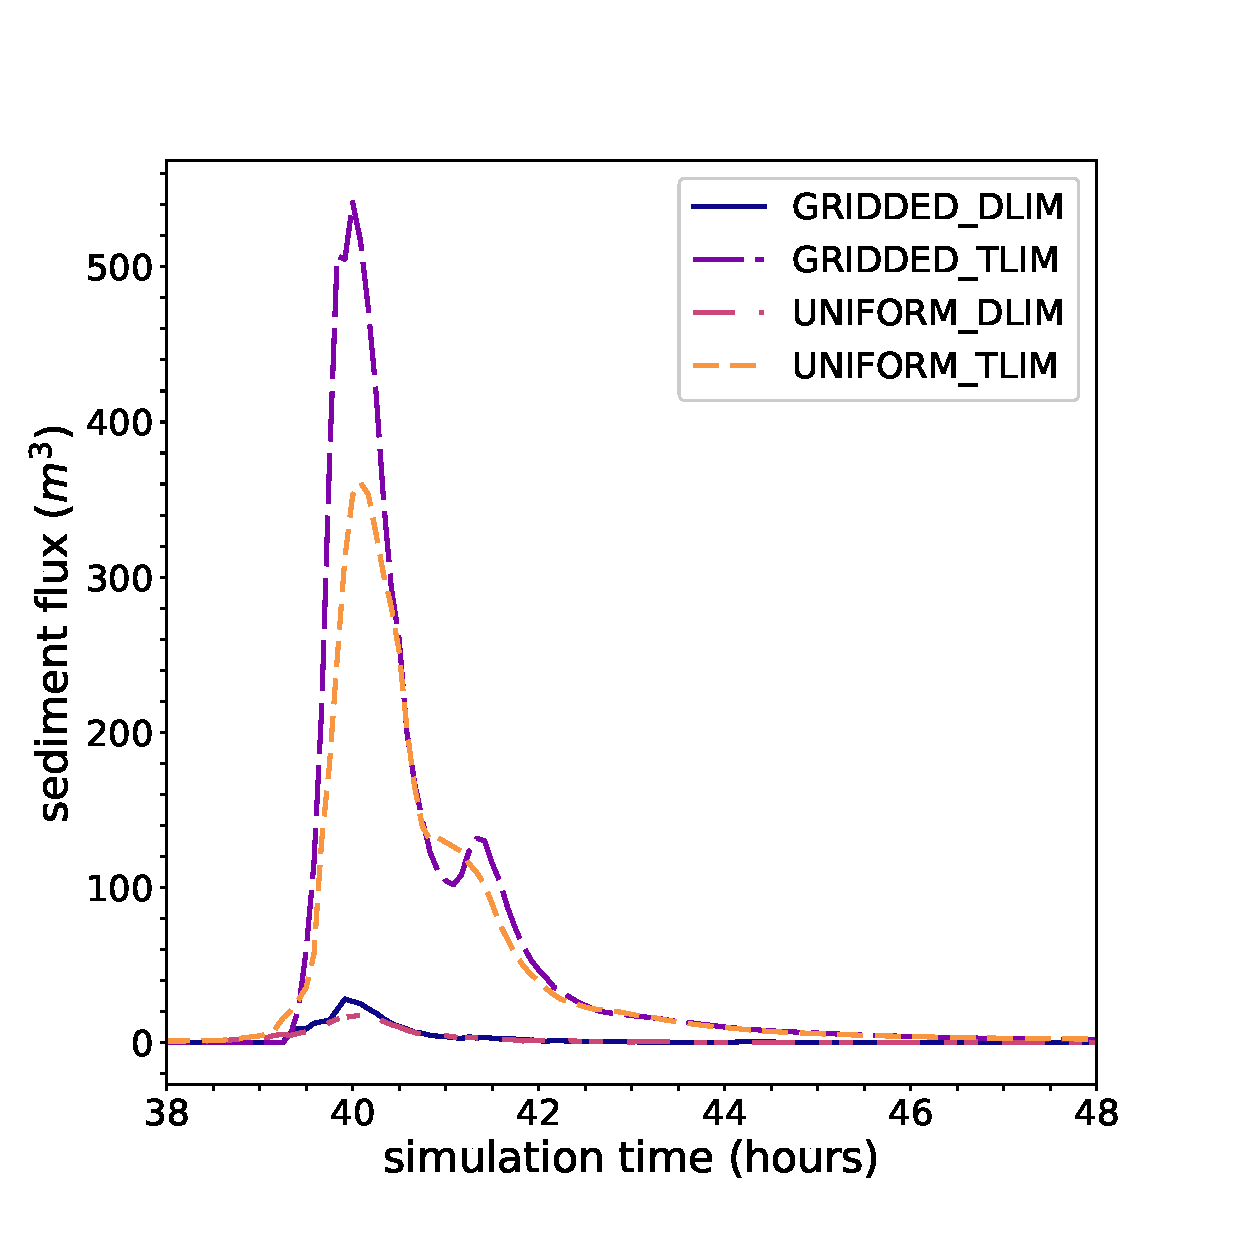
\includegraphics[width=14cm]{chp06_figures_scripts/figure_boscastle_sedigraph_ensemble.eps}
\caption{Boscastle sediment flux (total sediment volume output per hour at catchment outlet for each erosion-enabled simulation of the 2004 Boscastle event listed in Table \ref{table_ensemble_experiments}.}
\label{fig_boscastle_sedigraph_ensemble}
\end{figure}

\begin{figure}[t]
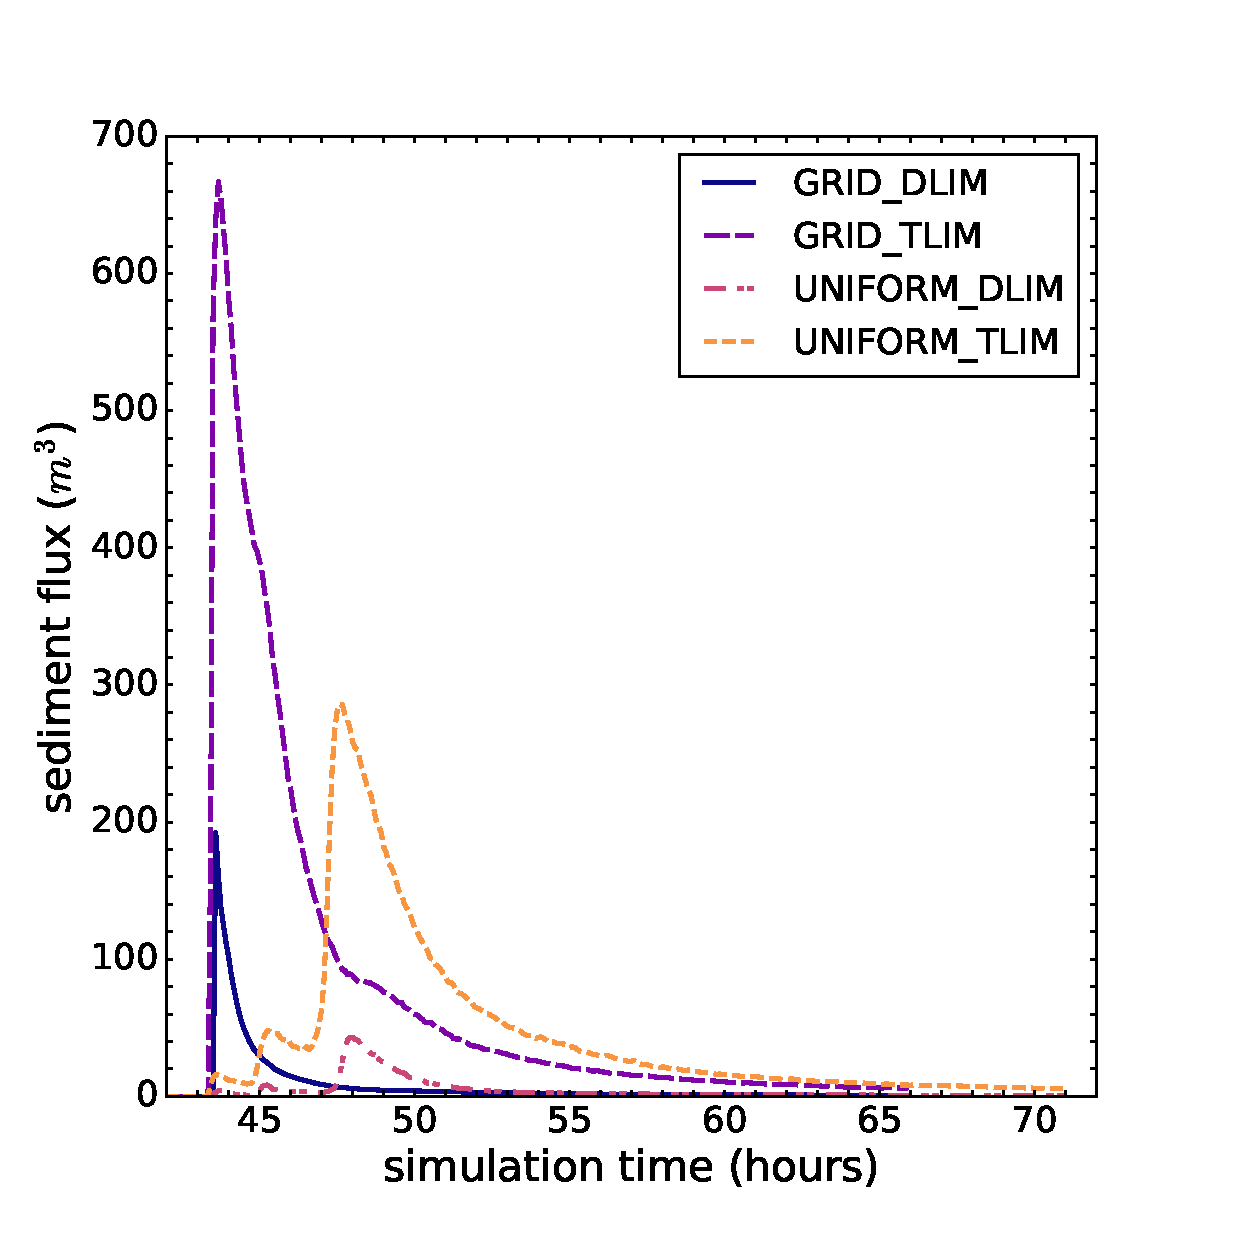
\includegraphics[width=14cm]{chp06_figures_scripts/figure_ryedale_sedigraph_ensemble.eps}
\caption{Ryedale sediment flux (Total sediment volume output per hour at catchment outlet) for each erosion-enabled simulation of the 2005 Ryedale event listed in Table \ref{table_ensemble_experiments}.}
\label{fig_ryedale_sedigraph_ensemble}
\end{figure}

% Describe planform variations in erosion and deposition
\subsection{Spatial variations in sediment and bedrock erosion}
The main spatial variation seen in sediment erosion is seen in river channels, where shear stresses require to initiate erosion and sediment transport are greatest due to the flow of water. The amount of erosion in each simulation was highly sensitive to parameterisation choice of the sediment erosion and transport law, with the choice of rainfall input data (gridded vs uniform) being only a secondary controlling factor on erosion amounts, all other factors being equal. This behaviour was seen on all simulations, in Figure \ref{fig_boscastle_2dplan_erosion_ensemble} and \ref{fig_ryedale_2dplan_erosion_ensemble}. 

To highlight the variation in erosion along the river channel, longitudinal profiles showing the average change in elevation after the storm are shown in Figures \ref{fig_boscastle_swath_tlim} and \ref{fig_ryedale_swath_tlim}. The longitudinal profile shows the variation in erosion along the main channel within each catchment, averaged along a 10 m wide swath centred on the midpoint of the channel. The swath profiling technique is adapted from \citep{hergarten2014extracting}. To reduce the number of points plotted along the swath profile, erosion is also averaged longitudinally, using bins spaced every 200m in the Ryedale catchment and every 50m in the Valency catchment.

% Swath profiles
% Boscastle TLIM
\begin{figure}[htb]
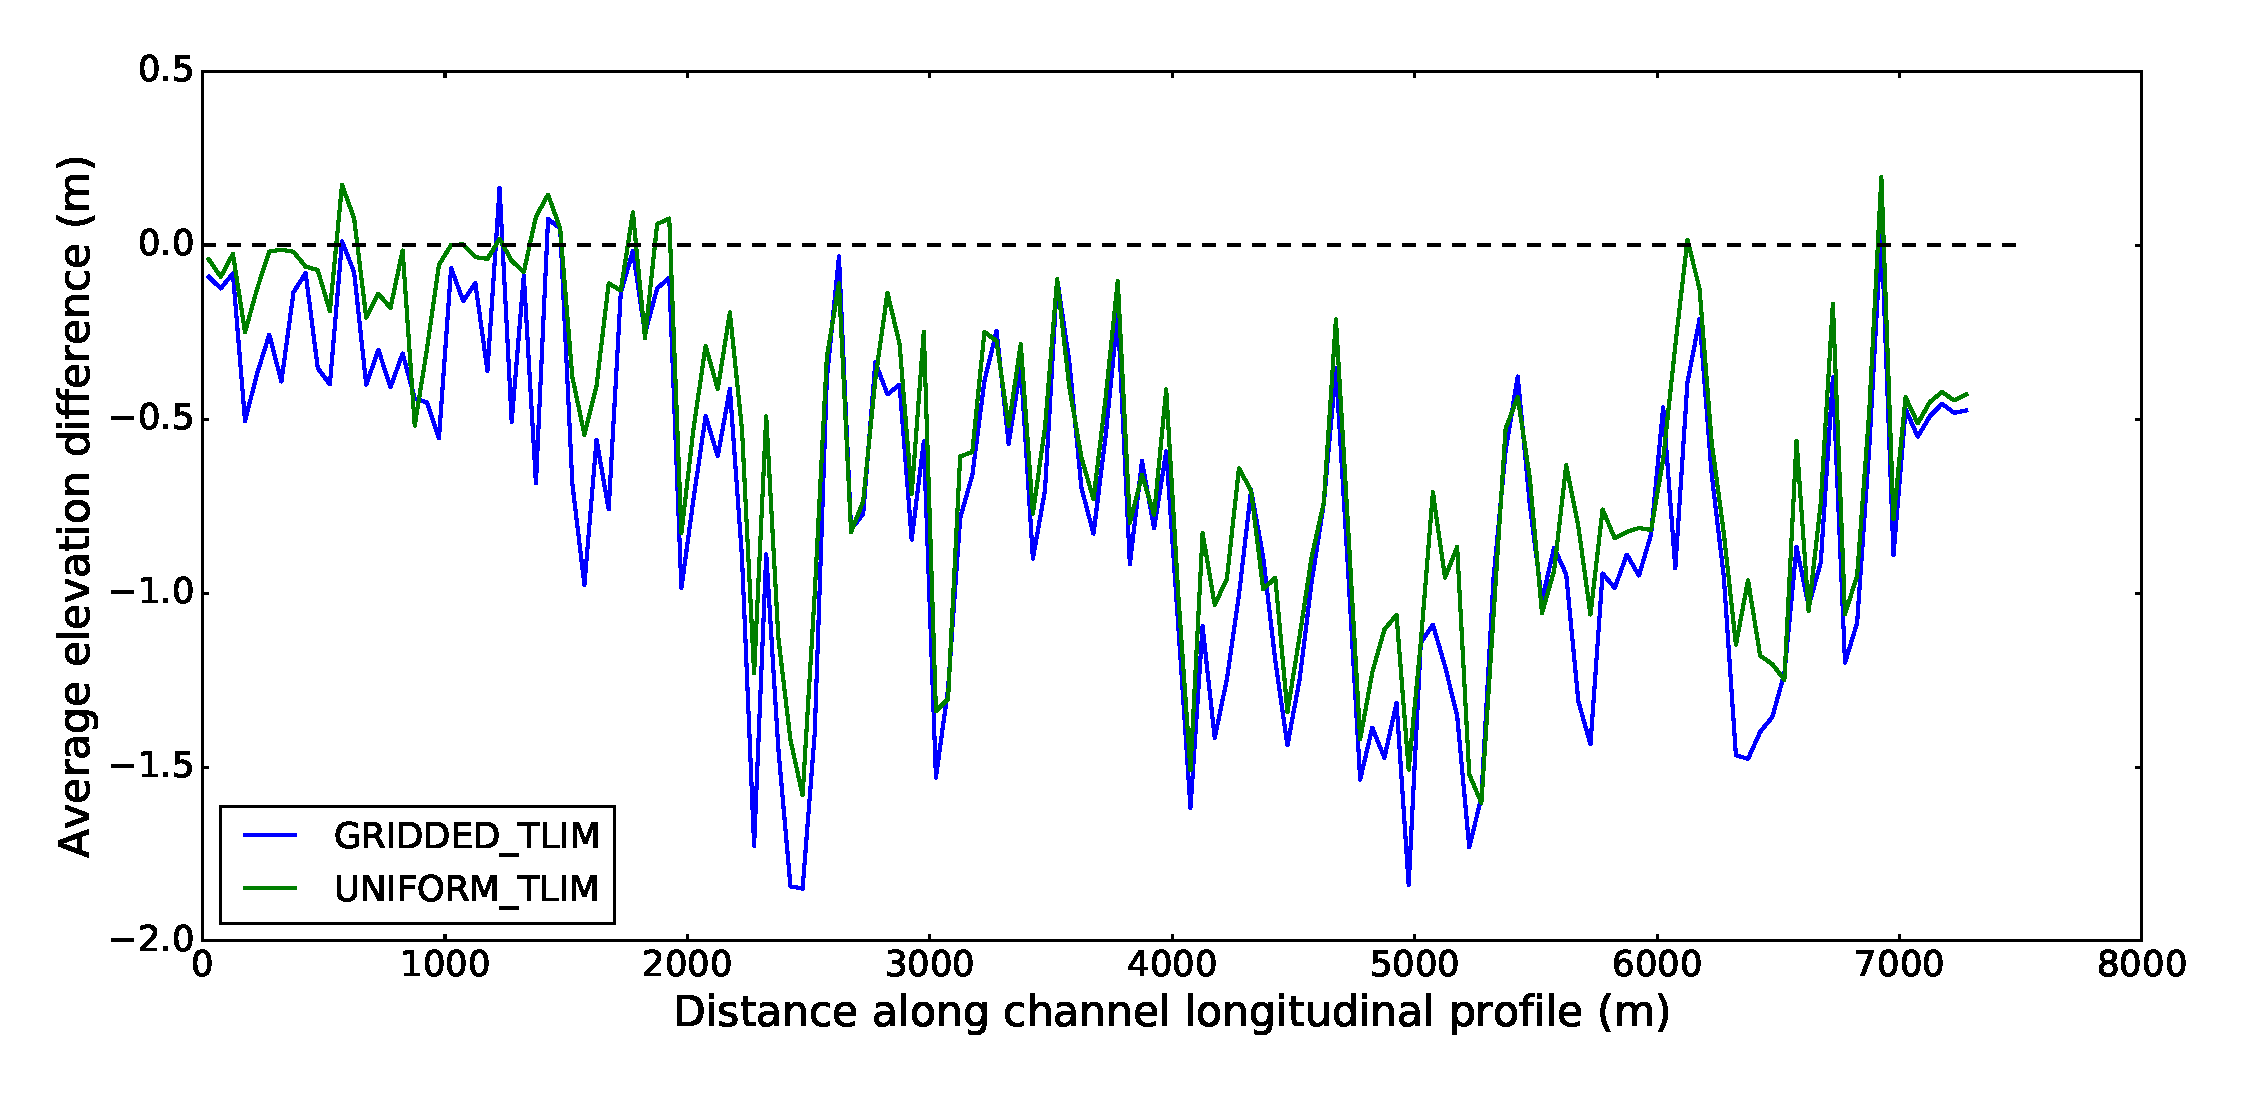
\includegraphics[width=14cm]{chp06_figures_scripts/fig_swath_profile_boscastle_erode_tlim.eps}
\caption{Channel averaged elevation difference along the main river channel in the Valency catchment. Simulation using the transport limited erosion parametrisation. Longitudinal profile is averaged over bins spaced every 50m. Transverse averaging (across the channel) is done over a 10m wide section centred on the channel midpoint. Results from the GRIDDED\_TLIM simulation shown in blue and the UNIFORM\_TLIM simulation shown in green.}
\label{fig_boscastle_swath_tlim}
\end{figure}

% Ryedale TLIM
\begin{figure}[htb]
\includegraphics[width=14cm]{chp06_figures_scripts/fig_swath_profile_ryedale_erode_tlim.eps}
\caption{Channel averaged elevation difference along the main river channel in the Valency catchment. Simulation using the transport limited erosion parametrisation. Longitudinal profile is averaged over bins spaced every 50m. Transverse averaging (across the channel) is done over a 10m wide section centred on the channel midpoint. Results from the GRIDDED\_TLIM simulation shown in blue and the UNIFORM\_TLIM simulation shown in green.}
\label{fig_ryedale_swath_tlim}
\end{figure}

Swath profiling of the Valency river channel (Boscastle) shows overall a net incision in the channel area, under transport-limited erosion parameterisation, with only small sections of the channel showing net sediment deposition (elevation increase) on average. Most incision is predicted to occur in the mid to upper reaches of the channel, with realtively little incision in the lowest reach of the catchment. The difference between gridded and uniform rainfall inputs shows a minimal difference along the main profile, though there is a slight tendency for the incision seen in the gridded rainfall input simulation to be higher in most places than the simulation using uniform input, with the difference in incision amounts of the order of tens of centimetres at most.

The swath profiling of the Rye river channel within the Ryedale catchment shows a large variation in incision and deposition rates within the catchment, though there is still an overall tendency for net incision. The magnitude of both incision and deposition is higher in the mid to upper reaches of the Rye river channel, similar to the pattern observed in the Valency river. The differences in average elevation changes are not as clearly distinguishable between the gridded and uniform rainfall input parameterisations, magnitudes of erosional and depositional peaks are slightly higher in the lower reaches of the river channel, but in the mid to upper reaches the differences are more varied. 
 
% OTHER SWATH PROFILES? DLIM, WIDER SWATH HALF WIDTH PERHAPS FOR RYEDALE?????
%
%

% Plan view erosion diff maps
\begin{sidewaysfigure}[t]
\includegraphics[width=25cm]{chp06_figures_scripts/figure_boscastle_erosion_diff_ensemble.png}
\caption{Boscastle. Erosion.}
\label{fig_boscastle_2dplan_erosion_ensemble}
\end{sidewaysfigure}

\begin{sidewaysfigure}[t]
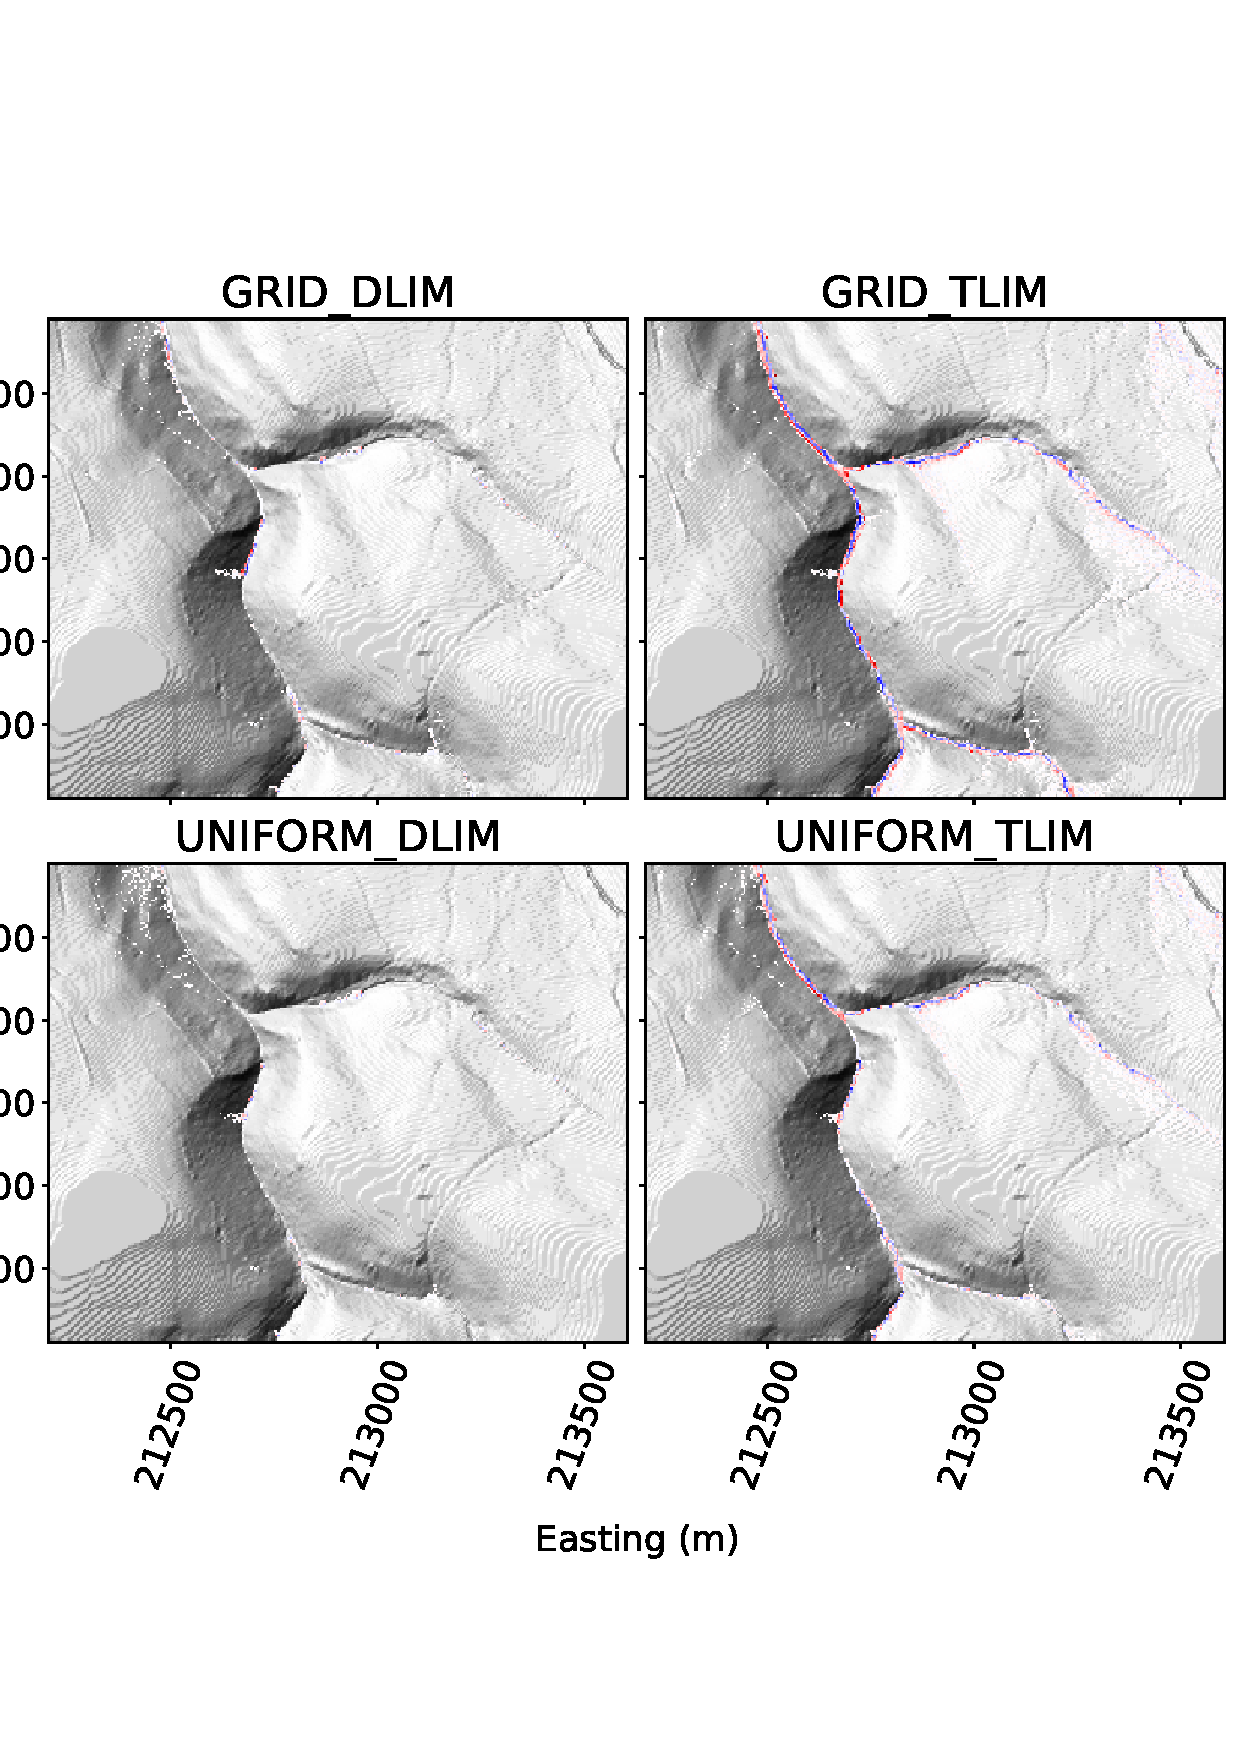
\includegraphics[width=18cm]{chp06_figures_scripts/figure_boscastle_erosion_diff_ensemble_SE.png}
\caption{Boscastle. Erosion. SE trib}
\label{fig_boscastle_2dplan_erosion_ensemble_SE}
\end{sidewaysfigure}

% Plan view erosion diff maps
\begin{sidewaysfigure}[t]
\includegraphics[width=25cm]{chp06_figures_scripts/figure_ryedale_erosion_diff_ensemble.png}
\caption{Ryedale. Erosion.}
\label{fig_ryedale_2dplan_erosion_ensemble}
\end{sidewaysfigure}

% Full extent erosion maps
\begin{sidewaysfigure}[t]
\includegraphics[width=25cm]{chp06_figures_scripts/boscastle_erodediff_grid_tlim.png}
\caption{Boscastle. Map of extent of catchment change in elevation greater than 0.02m. Change in elevation shown after 72 hours of model simulation using gridded rainfall and the transport limited erosion law. (GRID\_TLIM)}
\label{fig_boscastle_erodediff_grid_tlim}
\end{sidewaysfigure}

\begin{sidewaysfigure}[t]
\includegraphics[width=25cm]{chp06_figures_scripts/boscastle_erodediff_uniform_tlim.png}
\caption{Boscastle. Map of extent of catchment change in elevation greater than 0.02m. Change in elevation shown after 72 hours of model simulation using uniform rainfall and the transport limited erosion law. (UNIFORM\_TLIM)}
\label{fig_boscastle_erodediff_uniform_tlim}
\end{sidewaysfigure}

% RYEDALE lower reaches
\begin{figure}[htb]
\includegraphics[width=16cm]{chp06_figures_scripts/fig_ryedale_lower_erodediff_grid_tlim.png}
\caption{Ryedale. Map of extent of catchment change in elevation greater than 0.02m. Change in elevation shown after 72 hours of model simulation using gridded rainfall and the transport limited erosion law. (GRIDDED\_TLIM)}
\label{fig_ryedale_erodediff_lower_grid_tlim}
\end{figure}

\begin{figure}[htb]
\includegraphics[width=16cm]{chp06_figures_scripts/fig_ryedale_lower_erodediff_uniform_tlim.png}
\caption{Ryedale. Map of extent of catchment change in elevation greater than 0.02m. Change in elevation shown after 72 hours of model simulation using uniform rainfall and the transport limited erosion law. (UNIFORM\_TLIM)}
\label{fig_ryedale_erodediff_lower_uniform_tlim}
\end{figure}

\section{Discussion}

As with hydrology and flood extent (Chapter \ref{chapter_flood_model_sensitivity}), sediment flux exhibits sensitivity to the input rainfall data resolution, but the more dominant sensitivity is to the sediment erosion parameterisation choice in the model. The set of erosion-enabled simulations in these experiments represented two end-members of sediment transport and erosion laws. The \textit{TLIM}-suffixed simulations representing a purely transport limited environment and the \textit{DLIM}-suffixed environment representing a purely detachment limited environment -- with the transport limited law simulations predicting much greater sediment flux and erosion than the detachment limited counterparts. In terms of sediment flux and erosion, the role of rainfall input data spatial resolution played only a secondary role in determining erosion amounts. The size of the catchment was less important in this respect, with even the smaller Boscastle catchment showing a marked sensitivity to the choice of erosion law.

\section{Conclusion}
Over long term landscape evolution, erosional processes in catchments are known to be sensitive to the spatial distribution of rainfall input.  This study has shown that catchment erosional processes are also sensitive to rainfall spatial distribution during the course of a single severe storm, and it is suggested that this is due to the spatial variation in shear stresses required brought on by heterogeneous rainfall inputs to the catchment system.  As sediment transport and erosional process are highly threshold dependent, this leads to erosional patterns that differ according to the pattern of rainfall input. In other words, in the simulation of landscape evolution processes at the catchment scale, the choice of whether to use a uniform value representing the rainfall input, or to use a spatially heterogeneous gridded rainfall data, can have a marked impact on the predicted sediment yields from the catchment. 
In terms of sediment yields, however, these experiments have shown that it is the choice of erosional parameterisation in the model, and not necessarily the resolution of rainfall input data, that has a first-order control on the total sediment yields from a catchment and the magnitude of river channel incision during a simulated event.

Stuff amount rarity of events. Catastrophism.

\subsection{Implications for longer-term landscape evolution}
The experiments presented in this chapter have focused on the hydrogeomorphic response to single severe storm events, events which produced floods with return periods of 1 in 330 years (Ryedale) and 1 in 1300 years (Boscastle). The amounts of river channel incision predicted as a result of these storms is comparable to that predicted by studies of landscape evolution on scales of 1000 years, for example a study of a similar upland river basin by \citep{coulthard2016sensitivity} predicted channel incision amounts of 0.5--5m over 1000 years. The experiments presented here, using the same sediment transport law, predicts comparable incision amounts of channel incision during a single storm. If the flood return periods are assumed to be broadly correct, these simulations suggest that the majority of sediment erosion occurs during rare but high magnitude flood events, rather than through gradual processes or more frequent but lower magnitude events.


